\chapter{Frontend}
\label{chap:frontend}

Frontend je část webové aplikace, která komunikuje přímo s uživatelem, posílá dotazy na služby backendu a zobrazuje uživateli výsledky.

\section{HTML5}

Historicky měli frontendoví weboví developeři na výběr mezi několika technologiemi. Proprietální řešení jako Adobe Flash, nebo Microsoft Silverlight byly dříve jsdnou z mála možností, jak vyvíjet složitější frontendové aplikace. Jejich místo dnes nahrazuje skupina otevřených standardů pod souhrným označením HTML5.

HTML5 je označení jednak pro nejnovější verzi standardu značkovacího jazyka HTML, jednak je to termín zastřešující další moderní webové technologie, jako je například CSS3. HTML5 poskytuje frontendovým vývojářům široké spektrum nových API. Bez proprietálních pluginů je dnes možné v modernch prohlížečích například přehrávat video, nebo vykreslovat 2D grafiku.

Další zlepšení, které frontendovým vývojářům zlehčuje práci, jsou nová verze standardu ECMAScript, což je standard jazyka JavaScript. JavaScript je nyní daleko produktivnější jazyk, než byl ještě před pár lety a může využívat více API ze standardu HTML5.

\section{JavaScriptové frameworky}

Jednotlivé webové prohlížeče se dlouhá léta lišily v implementaci JavaScriptu do takové míry, že pro podporu více prohlížečů bylo použití nějakého frameworku, který sjednocuje API téměř nezbytné. Dnes už do značné míry nejsou při vývoji frontendu frameworku nezbytné, ale stále jsou velmi užitečné.

\subsection{jQuery}
Nejpopulárnějším frameworkem současnosti je jQuery. Ten nabízí jednoduché rozhraní pro práci s DOM a javascriptovými událostmi a pro velké množství menších webových aplikací je dostačující. Ve větších aplikacích se začne projevovat nižší výkon aplikace používající jQuery a také obtížné odstraňování chyb v aplikacu, debuggování.Například můžeme pomocí jQuery chtít přidat CSS třídu \uv{red} HTML elementu s id \uv{okno}

\begin{lstlisting}
  $("#okno").addClass("red");
\end{lstlisting}

Tento kód proběhne bez nahlášené chyby i v případě, že žádný element s id \uv{okno} neexistuje, nebo když uděláme překlep v zápisu řetězce. Pokud chce web knihovnu jQuery, musí ji celou nejdříve stáhnout. Aktuální verze $1.11.1$ má velikost téměř 100 KB. Knihovna jQuery je použita v implementaci anotačního rozhraní popsaném v Kapitole \ref{chap:rozhrani}.

\subsection{Google Closure}
Jiný přístup k vývoji frontendových aplikací přináší Google. Pro svou první webovou aplikaci Gmail vyvinul sadu nástrojů, kterou později vydal jako sadu nástrojů Google Closure. Kromě služby Gmail používá Google sadu nástrojů i pro vývoj Google Vyhledávání, Google Map, nebo Google Dokumentů. Skládá se ze tří částí - Closure Compiler, Closure Library a Closure Templates.

Closure Library je javascriptová knihovna funkcí pro práci s DOMem, javascriptovýmy událostmi, matematickými výpočty a spoustou dalších věcí, které webový programátor může využít.

Closure Compiler je minifikátor javascriptového kódu. Minifikace javascriptového kódu je důležitá, protože snižuje množství dat, které musí webová stránkapřed spuštěním stáhnout. Compiler odstraňuje nedůležité mezery v kódu, odstraňuje funkce, které nejsou volány, přejmenovává názvy funkcí a proměnných na co nejkratší řetězce a v ADVANCED módu se snaží i o pokročilejší optimalizace kódu (například inlineing funkcí). Nejlepích výsledků dosahuje s použitím typových anotací. Anotace jsou silně inspirovány jazykem Java a díky nim lze z JavaScriptu vytvořit typovaný objektový jazyk s privátními metodami, nebo dědičností tříd. Closure Compiler tyto anotace vyhodnocuje a vrací chyby a varování, podobně jako jiné kompilované jazyky. To umožňuje snadněji psát spolehlivý javascriptová kód.

Třetí částí sady nástrojů Google Closure jsou Closure Templates, šablonovací systém pro JavaScript a Javu. Pomocí Closure Templates se snadno vytváří zanořené HTML šablony se zadanými parametry. Closure Templates automaticky ošetřují vstupní data, což zabraňuje bezpečnostním útokům na stránku.

Částí Templates a Compiler jdou použít odděleně v jakémkoliv Javascriptovém projektu. Používat Closure Library bez Compileru nedává příliš smysl, uživatel by při návštěvě webu musel stahovat ohromné množství zbytečných dat.

Frontendová část aplikace je napsána s použitím všech částí Google Closure. Díky tomu je frontendová část serveru tvořena jediným javascriptovým souborem velikosti 65 KB.

\section{CSS}

CSS ve verzi 3 přidává mnoho nových vlastností, které jdou HTML elementům přiřadit. Nejviditelnějšími jsou kulaté okraje, nebo stínování. Pro programátory je zajímavá vlastnost \uv{calc} pomocí níž lze zadat hodnoty v CSS jako výpočet. Pokud například chceme, aby se element roztáhl na polovinu obrazovky a měl vedle sebe ještě 10 pixelů místo, nastavíme mu vlastnost

\begin{lstlisting}
 width: calc("50% - 10px");
\end{lstlisting}

Bez této vlastnosti šlo dříve podobné chování simulovat pouze pomocí JavaScriptu. Vlastnosti jako \uv{calc} umožňují programátorům snadněji psát responzivní aplikace. To jsou takové aplikace, které se dobře přizpůsobují velikosti okna prohlížeče. Responzivnost webových aplikací začala být důležitá zejména s rozvojem mobilních technologií. Stále větší počet uživatelů přistupuje na weby ze svých mobilních telefonů, nebo tabletů a tito uživatelé chtějí mít při používání aplikace podobný komfort jako na při používání na počítači. Při vývoji frontendu 

\section{Uživatelské rozhraní}

Uživatelské rozhraní aplikace tvoří jediná webová stránka. Uživatel pracuje ve dvou základních režimech --- vyhledávání obrázků a detail obrázku.

\subsection{Rozhraní pro vyhledávání obrázků}

\begin{figure}[h]
  \centering
  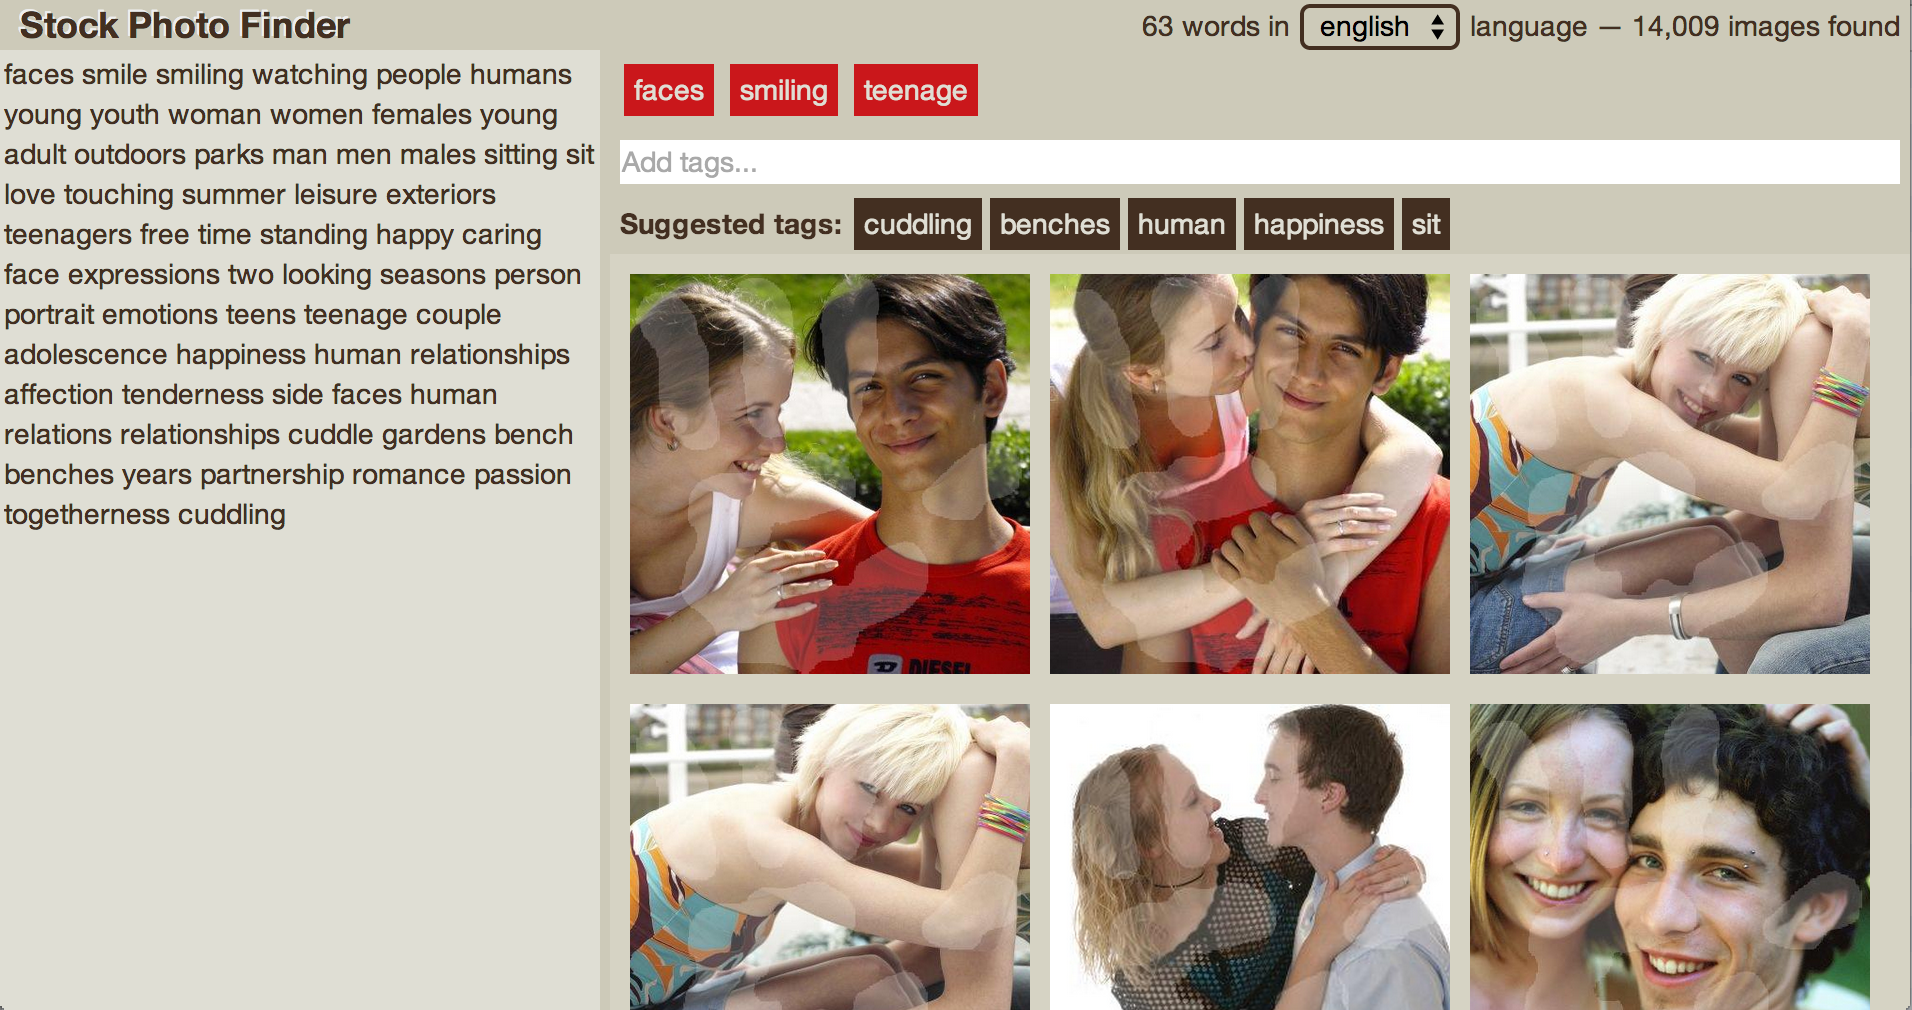
\includegraphics[width=150mm]{ui1.eps}
  \caption{Uživatelské rozhraní pro vyhledávání ilustračních obrázků.}
  \label{fig:ui1}
\end{figure}

Rozhraní pro vyhledávání obrázků slouží uživateli k vyhledání obrázku podle jím zadaných textových parametrů. Ukázka rozhraní je na Obrázku \ref{fig:ui1}. Rozhraní lze rozdělit na 3 části --- záhlaví, levý panel a pravý panel. Přetahováním myší za oblast rozdělující levý a pravý panel je možné měnit jejich velikost.

V levém panelu se nachází oblast na vložení textu. Zde může uživatel vložit text článku ke kterému hledá ilustrační obrázky. Uživatelské rozhraní samo detekuje změny v textu a zobrazuje ilustrační obrázky bez toho, aby uživatel musel stisknout tlačítko.

Záhlaví obsahuje statistiky o počtu nalezených obrázků a počtu slov v textu. V rozbalovacím menu je vybrán automaticky detekovaný jazyk vstupního textu. Uživatel má možnost tento jazyk manuálně změnit.

Pravý panel je rozdělen na horní a spodní část. Ve spodní části jsou zobrazeny náhledy nalezených obrázků. Po najetí myší nad obrázek se zobrazí u obrázku i jeho název a klíčová slova z datasetu Profimedie. Celý levý panel funguje na principu \uv{nekonečného} skrolování --- po naskrolování na spodek panelu se načtou další obrázky z výsledků vyhledávání (pokud ještě nějaké nezobrazené výsledky vyhledávání existují). Po kliknutí na obrázek myší se zobrazí rozhraní s detailem obrázku.

Horní část pravého panelu obsahuje komponenty pro explicitní zadání klíčových slov, které uživatel požaduje u vyhledaných obrázků. Klíčová slova může uživatel přidat buď přímo zápisem do textového vstupu \uv{Add tags...} a stisknutím klávesy \lstinline{ENTER}, nebo může kliknout na některé z detekovaných klíčových slov pod textovým vstupem. Nad textovým vstupem se na červeném pozadí nachází explicitně požadovaná klíčová slova. Kliknutím na explicitně vybrané slovo se slovo odstraní z požadované množiny klíčových slov.

\subsection{Rozhraní pro detail obrázku}

\begin{figure}[h]
  \centering
  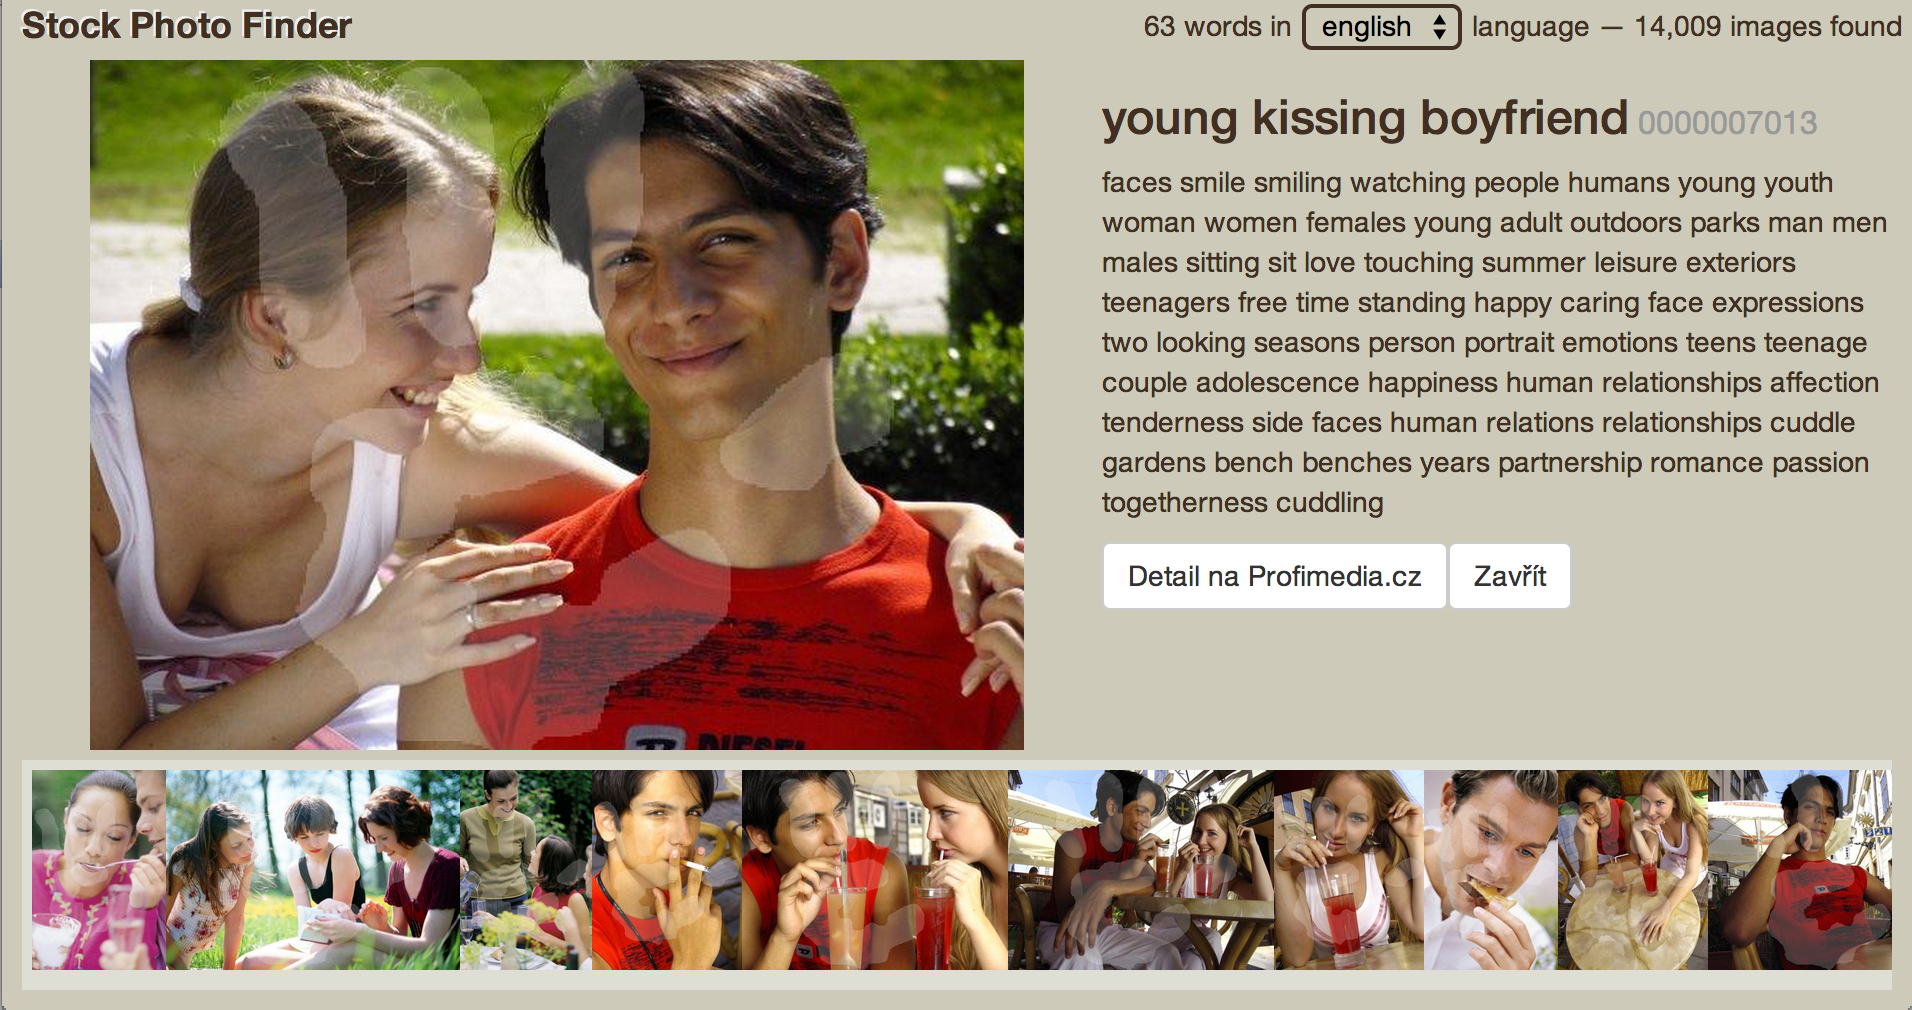
\includegraphics[width=150mm]{ui2.eps}
  \caption{Uživatelské rozhraní s detailem obrázku.}
  \label{fig:ui2}
\end{figure}

Rozhraní s detailem obrázku vyvolá uživatel kliknutím na obrázek ve vyhledávacím rozhraní. Ukázka tohoto rozhraní je na Obrázku \ref{fig:ui2}.

V levé horní části vidí uživatel celý obrázek. Pravá horní část rozhraní obsahuje textove popisky obrázku v datasetu Profimedie --- název, id a klíčová slova. Pod nimi jsou dvě tlačítka. První je odkazem na detail obrázku na webu Profimedia, druhým tlačítkem uživatel zavře detail obrázku a vrátí se zpět do vyhledávacího rozhraní.

Ve spodní části rozhraní je seznam podobných obrázků k obrázku v detailu. Po kliknutí na některý z podobných obrázků se zobrazí detail příslušného obrázku.

\section{Závěr}

Frontend aplikace zpřístupňuje uživateli prohledávání datasetu Profimedie. Při vývoji byl kladen důraz na uživatelskou přívětivost a použití nejmodernějších frontendových technologií. V celém rozhraní jsou tak například pouze dvě tlačítka. Rozhraní se samo přizpůsobuje velikosti obrazovky uživatele. Pro uživatele komfortní by měla být i automatická detekce jazyku vloženého textu, nebo možnost měnit velikost panelů ve vyhledávacím rozhraní.




